
\subsection*{\textbf{Question 1.e)}}
\begin{quote}

\textbf{Problem}
\begin{quote}
Download the dataset. The dataset contains 10 sets of random numbers. Compare these 10 sets with your Gaussian pseudo random numbers and make the plot of the probabilities as in either of the previous two exercises (your choice). Which random number arrays is/are consistent with a Gaussian random numbers with $\sigma = 1$ and $\mu = 0$
\end{quote}

\textbf{Solution} 
\begin{quote}
The distributions are compared by performing the KS-test 2 (2 sample distributions). The KS-test 2 has to be applied to 10 columns. The random numbers that are compared with the column data are as result only generated once (i.e each column is  compared with the same random numbers). This was done to save computation time.  The code that contains the implementation of the ks-test 2 can be found on page 22.  The code that generates the plots and the generated plots can be found below.
\\
\\
The plots show that there is only one column which might be\footnote{A p-value only shows statistical evidence against the null hypothesis, it isn't a measure of how good the null hypothesis is.} a normal distribution with $\sigma = 1$ and $\mu = 0$. This is column 4 (index 3, see figure 12 on page 15). In all other plots the p-value drops and stays below $ p = 0.05$ when including all samples, which indicates that their is enough statistical evidence to reject the hypothesis that they follow a normal distribution with $\sigma = 1$ and $\mu = 0$. 

\end{quote}
\newpage

\textbf{Code - Plots}

\begin{quote}
The code for generating the 10 plots. 
\lstinputlisting[firstline=237,lastline=290]{./Code/assigment_1.py}
\end{quote}
\newpage


\textbf{Code - Output plot(s)} \\
\textbf{Note:} Expect very similar captions for the upcoming 10 plots.
\begin{quote}
\begin{figure}[!ht]
\centering
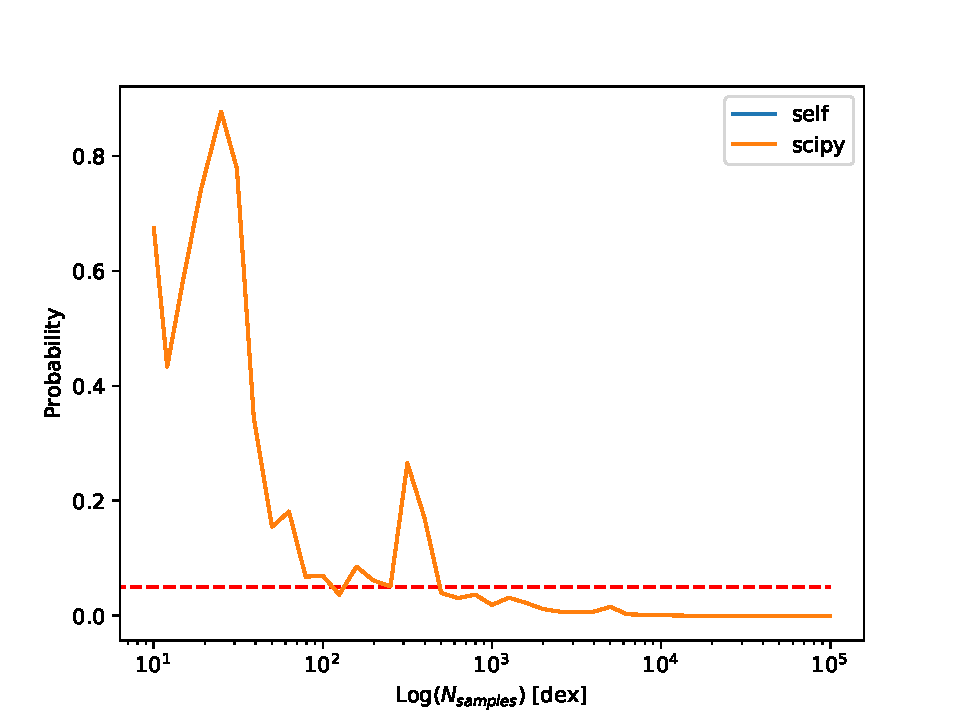
\includegraphics[width=14cm, height=8cm]{./Plots/1e_plot_column_0.pdf}
\caption{The P-value produced by performing the KS-test2 for a normal distribution with $\mu = 0$ and $\sigma = 1$ on the \textbf{first} column.  The red line indicates the line of $ p = 0.05$. A point \textbf{below} there  line would suggests that there is enough statistical evidence to reject the (null) hypothesis that the data is normal distributed. The plot shows that the p-value drops below 0.05 when including all samples. There is thus enough statistical evidence to reject the hypothesis that this column is normal distributed with $\mu = 0$ and $\sigma = 1$.}
\end{figure}

\begin{figure}[!ht]
\centering
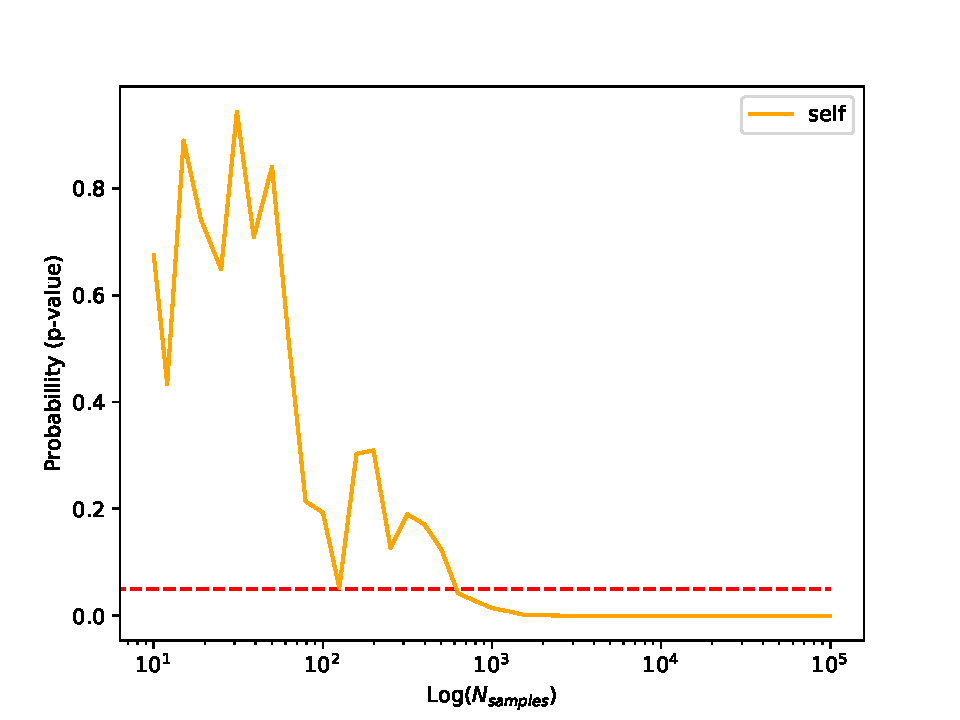
\includegraphics[width=14cm, height=8cm]{./Plots/1e_plot_column_1.pdf}
\caption{The P-value produced by performing the KS-test2 for a normal distribution with $\mu = 0$ and $\sigma = 1$ on the \textbf{second} column.  The red line indicates the line of $ p = 0.05$. A point \textbf{below} there  line would suggests that there is enough statistical evidence to reject the (null) hypothesis that the data is normal distributed. The plot shows that the p-value drops below 0.05 when including all samples. There is thus enough statistical evidence to \textbf{reject} the hypothesis that this column is normal distributed with $\mu = 0$ and $\sigma = 1$.}
\end{figure}
\newpage

\begin{figure}[!ht]
\centering
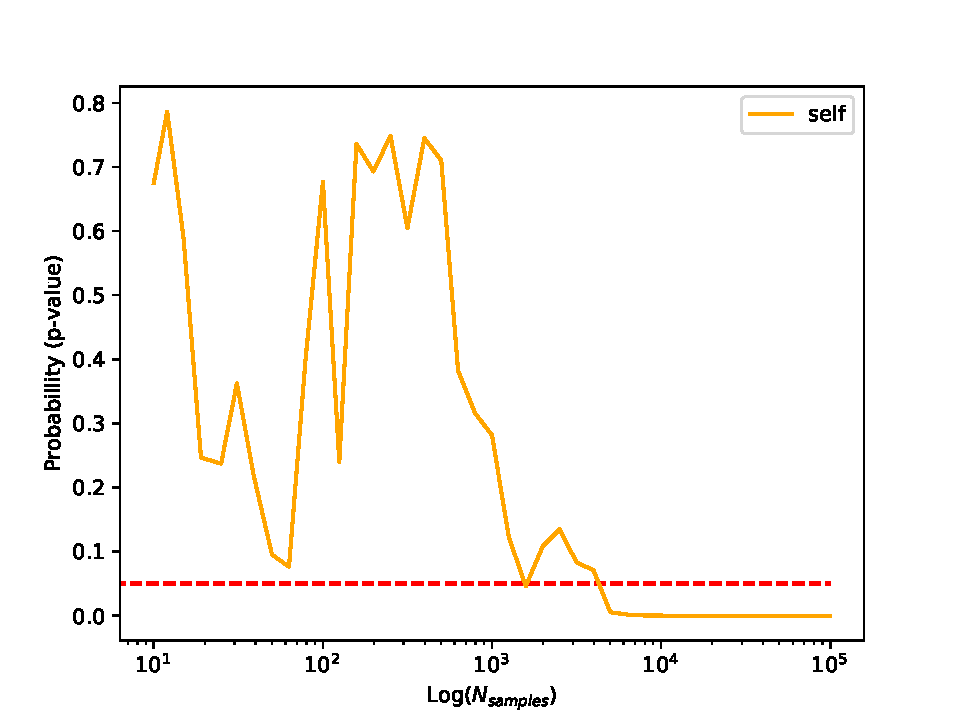
\includegraphics[width=14cm, height=8.5cm]{./Plots/1e_plot_column_2.pdf}
\caption{The P-value produced by performing the KS-test2 for a normal distribution with $\mu = 0$ and $\sigma = 1$ on the \textbf{third} column.  The red line indicates the line of $ p = 0.05$. A point \textbf{below} there  line would suggests that there is enough statistical evidence to reject the (null) hypothesis that the data is normal distributed. The plot shows that the p-value drops below 0.05 when including all samples. There is thus enough statistical evidence to \textbf{reject} the hypothesis that this column is normal distributed with $\mu = 0$ and $\sigma = 1$.}
\end{figure}

\begin{figure}[!ht]
\centering
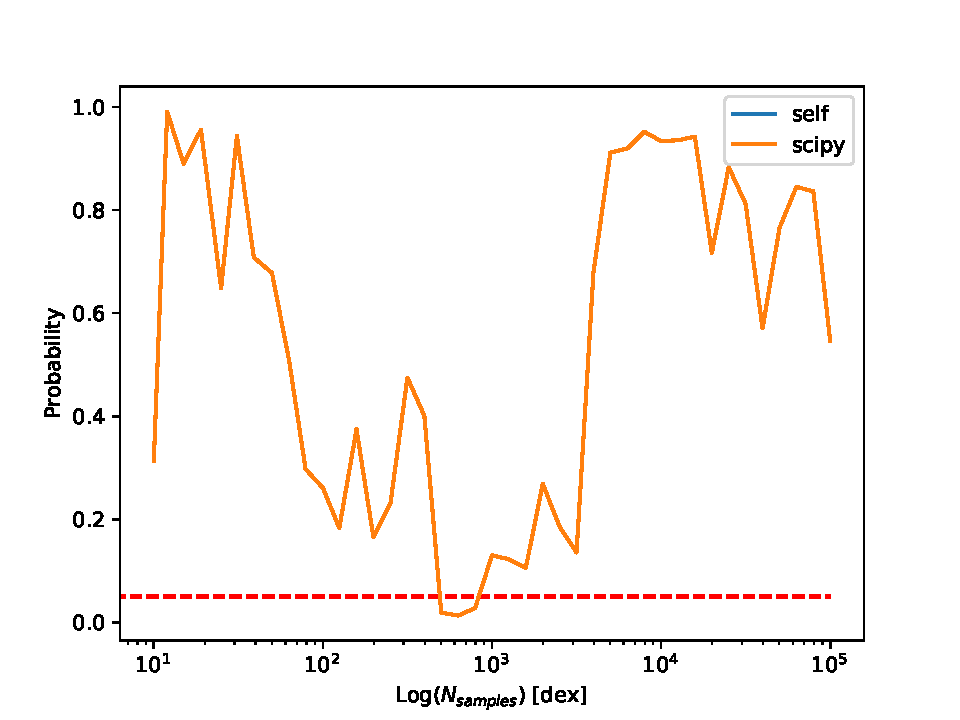
\includegraphics[width=14cm, height=8.5cm]{./Plots/1e_plot_column_3.pdf}
\label{FIG:Good}
\caption{The P-value produced by performing the KS-test2 for a normal distribution with $\mu = 0$ and $\sigma = 1$ on the \textbf{fourth} column.  The red line indicates the line of $ p = 0.05$. A point \textbf{below} there  line would suggests that there is enough statistical evidence to \textbf{reject} the (null) hypothesis that the data is normal distributed. The plot shows that the p-value drops below 0.05 only between $500-1000$ samples. In all other cases it passes the KS-test. The most important point in this plot is the p-value when all samples are included. It can be clearly seen that this point isn't below the red line. The plot therefore suggests that the given c olumn might( see footnote 2 on page 12) be a Gaussian with $\mu = 0$ and $\sigma =1$.  }
\end{figure}
\newpage

\begin{figure}[!ht]
\centering
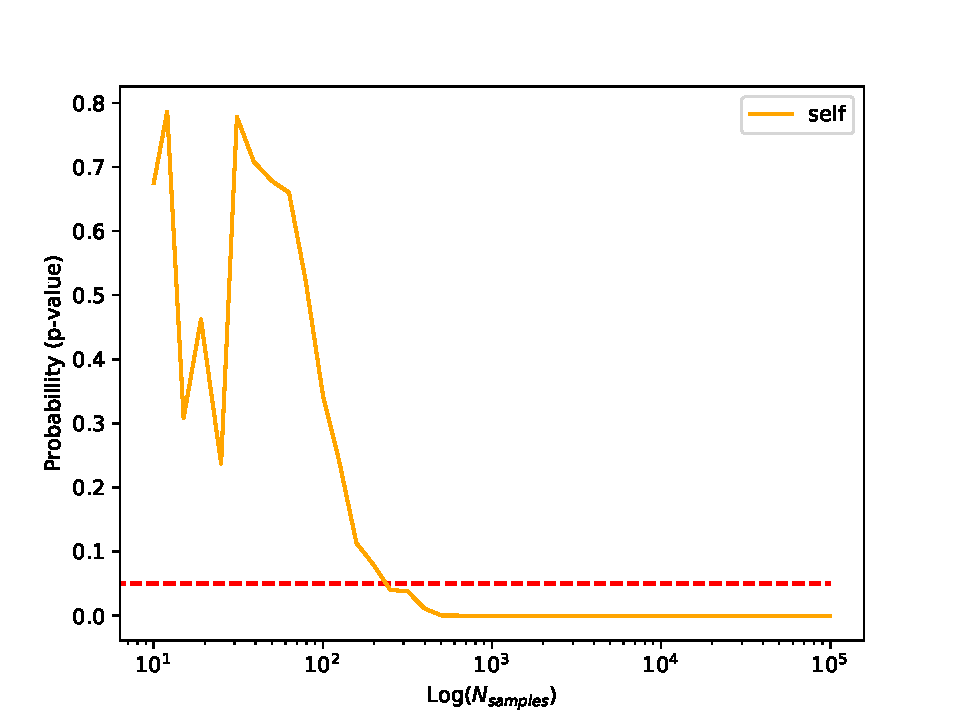
\includegraphics[width=14cm, height=8.5cm]{./Plots/1e_plot_column_4.pdf}
\caption{The P-value produced by performing the KS-test2 for a normal distribution with $\mu = 0$ and $\sigma = 1$ on the \textbf{fifth} column.  The red line indicates the line of $ p = 0.05$. A point \textbf{below} there  line would suggests that there is enough statistical evidence to reject the (null) hypothesis that the data is normal distributed. The plot shows that the p-value drops below 0.05 when including all samples. There is thus enough statistical evidence to reject the hypothesis that this column is normal distributed with $\mu = 0$ and $\sigma = 1$.}
\end{figure}


\begin{figure}[!ht]
\centering
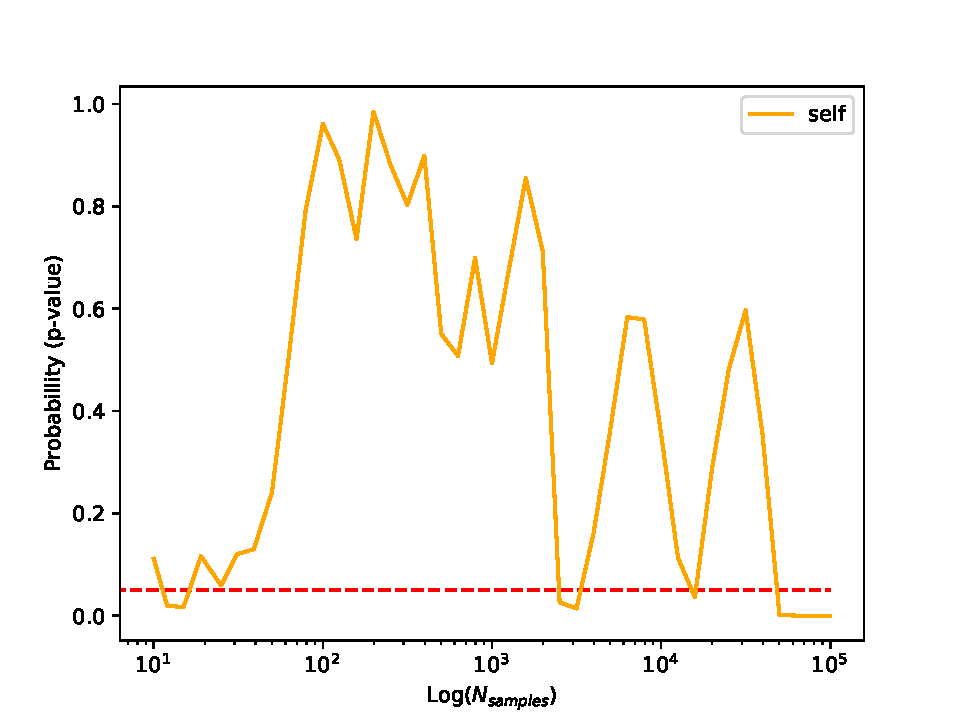
\includegraphics[width=14cm, height=8.5cm]{./Plots/1e_plot_column_5.pdf}
\caption{The P-value produced by performing the KS-test2 for a normal distribution with $\mu = 0$ and $\sigma = 1$ on the \textbf{sixth} column.  The red line indicates the line of $ p = 0.05$. A point \textbf{below} there  line would suggests that there is enough statistical evidence to reject the (null) hypothesis that the data is normal distributed. The plot shows that the p-value drops below 0.05 and stays there when including more than halve of the samples. The most important part of the figure is the part that includes most samples. There is thus enough statistical evidence to reject the hypothesis that this column is normal distributed with $\mu = 0$ and $\sigma = 1$.}
\end{figure}

\newpage

\begin{figure}[!ht]
\centering
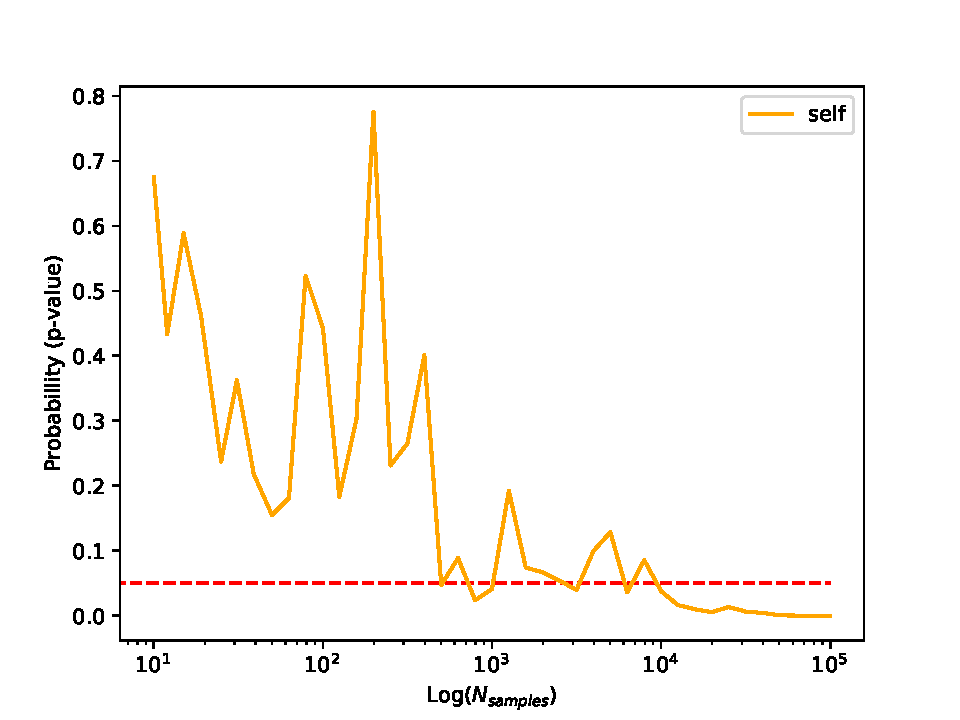
\includegraphics[width=14cm, height=8.5cm]{./Plots/1e_plot_column_6.pdf}
\caption{The P-value produced by performing the KS-test2 for a normal distribution with $\mu = 0$ and $\sigma = 1$ on the \textbf{seventh} column.  The red line indicates the line of $ p = 0.05$. A point \textbf{below} there  line would suggests that there is enough statistical evidence to reject the (null) hypothesis that the data is normal distributed. The plot shows that the p-value drops below 0.05 when including all samples. There is thus enough statistical evidence to reject the hypothesis that this column is normal distributed with $\mu = 0$ and $\sigma = 1$.}
\end{figure}


\begin{figure}[!ht]
\centering
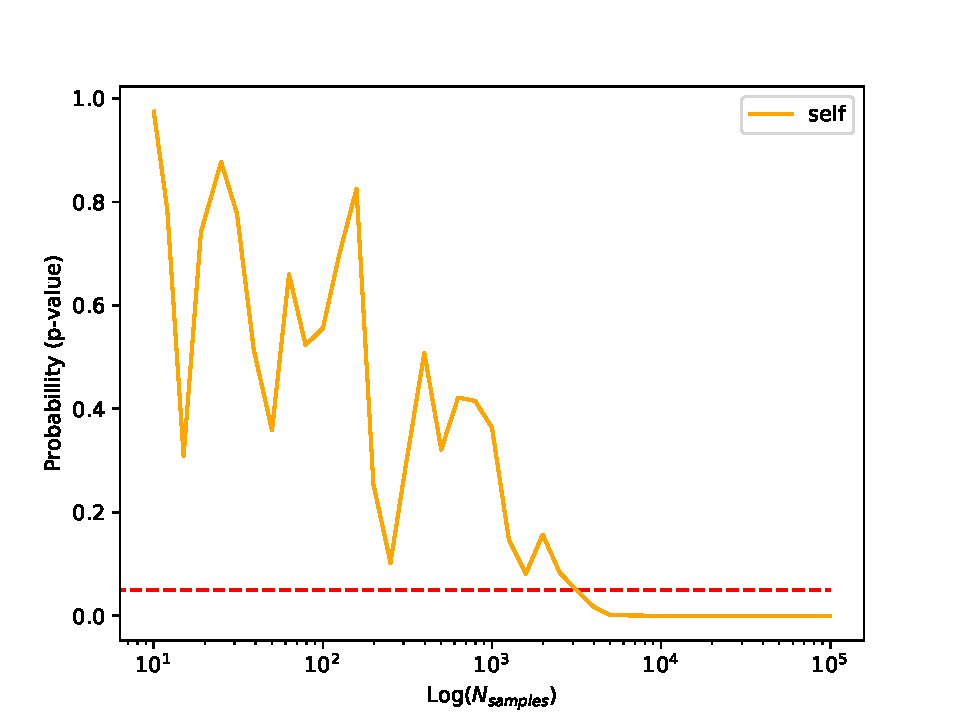
\includegraphics[width=14cm, height=8.5cm]{./Plots/1e_plot_column_7.pdf}
\caption{The P-value produced by performing the KS-test2 for a normal distribution with $\mu = 0$ and $\sigma = 1$ on the \textbf{eight} column.  The red line indicates the line of $ p = 0.05$. A point \textbf{below} there  line would suggests that there is enough statistical evidence to reject the (null) hypothesis that the data is normal distributed. The plot shows that the p-value drops below 0.05 when including all samples. There is thus enough statistical evidence to reject the hypothesis that this column is normal distributed with $\mu = 0$ and $\sigma = 1$.}
\end{figure}

\newpage

\begin{figure}[!ht]
\centering
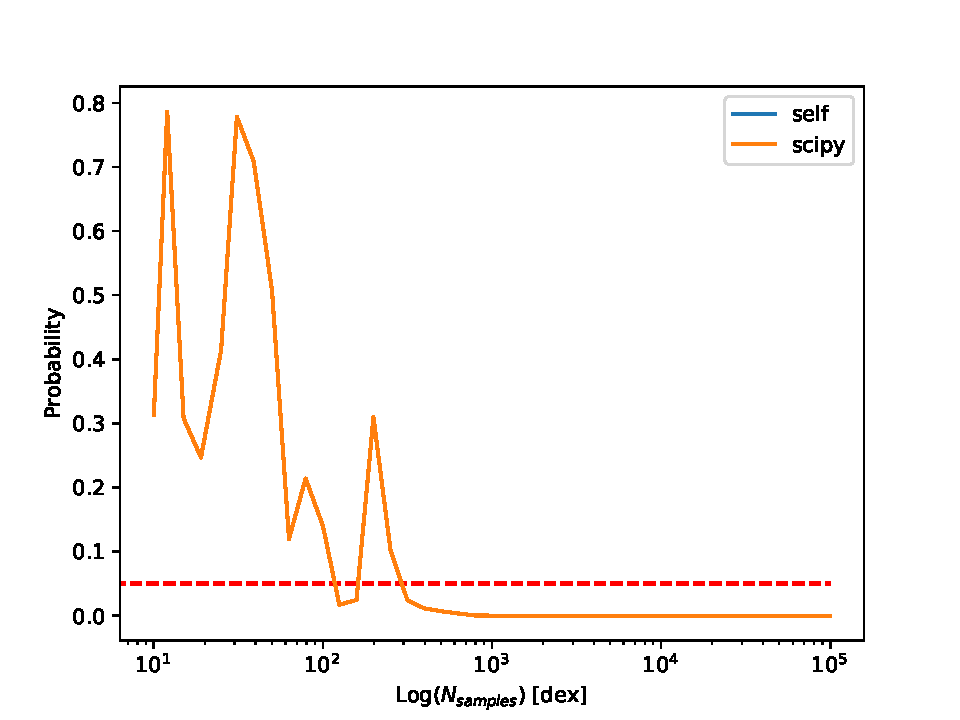
\includegraphics[width=14cm, height=8.5cm]{./Plots/1e_plot_column_8.pdf}
\caption{The P-value produced by performing the KS-test2 for a normal distribution with $\mu = 0$ and $\sigma = 1$ on the \textbf{ninth} column.  The red line indicates the line of $ p = 0.05$. A point \textbf{below} there  line would suggests that there is enough statistical evidence to reject the (null) hypothesis that the data is normal distributed. The plot shows that the p-value drops below 0.05 when including all samples. There is thus enough statistical evidence to reject the hypothesis that this column is normal distributed with $\mu = 0$ and $\sigma = 1$.}
\end{figure}

\begin{figure}[!ht]
\centering
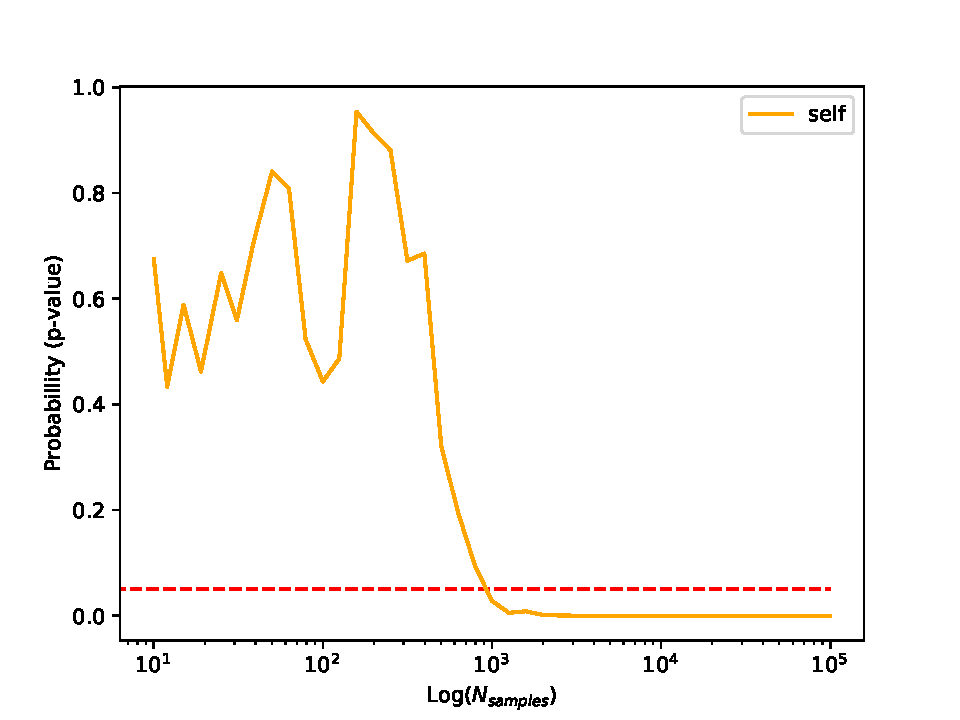
\includegraphics[width=14cm, height=8.5cm]{./Plots/1e_plot_column_9.pdf}
\caption{The P-value produced by performing the KS-test2 for a normal distribution with $\mu = 0$ and $\sigma = 1$ on the \textbf{tenth} column.  The red line indicates the line of $ p = 0.05$. A point \textbf{below} there  line would suggests that there is enough statistical evidence to reject the (null) hypothesis that the data is normal distributed. The plot shows that the p-value drops below 0.05 when including all samples. There is thus enough statistical evidence to reject the hypothesis that this column is normal distributed with $\mu = 0$ and $\sigma = 1$.}
\end{figure}
\end{quote}



\end{quote}

\newpage

%\textbf{Code - output } 
%\begin{quote}
% The code that produces the output.
%\lstinputlisting{./code/assigment1_a.py}
%\end{quote}

%\textbf{Code - helper } 
%\begin{quote}
%The code for the Poisson distribution and the factorial function.  
%\lstinputlisting[firstline=2,lastline=46]{./code/mathlib/utils.py}
%\end{quote}


%\textbf{Output}
%\begin{quote}
%The output produced by \textsf{/code/assigment1\_ a.py} 
%\lstinputlisting{./output/assigment1_a_out.txt}
%\end{quote}
\newpage











